\chapter{Diagramas de Ellingham e metalurgia}\label{ch:b2:ellingham}

Um alto-forno transforma rocha vermelha em ferro líquido com coque e ar
quente, ao ritmo de milhares de toneladas por dia. Nenhum forno desse tipo
jamais produzirá alumínio, magnésio ou titânio, embora o carbono seja igualmente
barato para eles. A maioria dos metais é encontrada no solo na forma de
óxidos, e obter um metal significa retirar seu oxigênio: quais redutores
conseguem fazê-lo, e a que temperatura, é uma questão de \omterm{def:b2:reaction-free-energy:gibbs-energy}{energias de Gibbs}
padrão. Em 1944, Harold Ellingham as traçou todas em um único gráfico, em
função da temperatura, cada uma para um mol de dioxigênio. O gráfico responde
num relance qual metal reduz qual óxido, por que o carbono vence a alta
temperatura e por que alguns metais precisam ser produzidos por eletrólise.

\begin{recall}
\Cref{ch:b2:reaction-free-energy}: $\Delta_r G^\circ = \Delta_r H^\circ -
T\Delta_r S^\circ$ e a \omterm{def:b2:reaction-free-energy:ellingham-approximation}{aproximação de Ellingham} (retas em $T$, exceto nas
mudanças de estado). \Cref{ch:b2:equilibrium-shifts}: $K^\circ$ a partir de
$\Delta_r G^\circ$, \omterm{def:b2:equilibrium-shifts:variance}{variância}, o fim de um equilíbrio quando uma fase
desaparece. O volume do 1.º ano: números de oxidação, pares redox, óxidos
básicos e ácidos. O volume escolar: os minérios.
\end{recall}

\begin{omfigure}
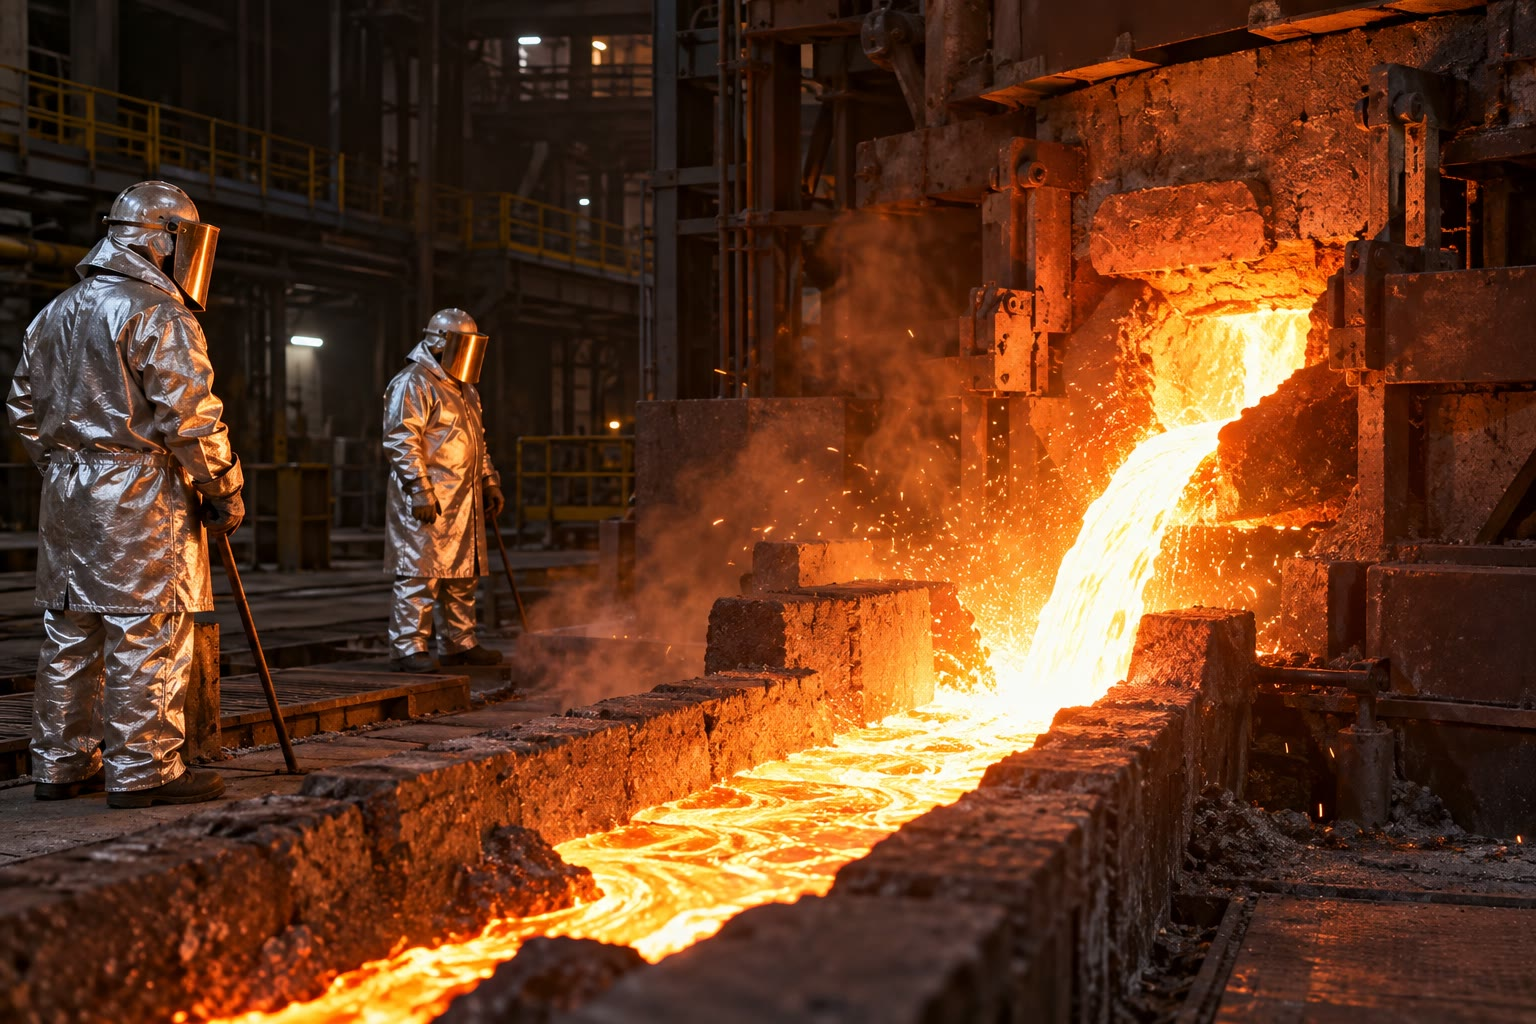
\includegraphics[width=0.62\linewidth]{images/book3/ai/b2-06-blast-furnace.jpg}

{\small A corrida de um alto-forno: o ferro líquido escorre por um canal
refratário, vigiado por operários em roupas que refletem o calor. A
temperatura e o gás no interior do forno são os que permitem ao monóxido de
carbono retirar o oxigênio do óxido de ferro.}
\end{omfigure}

\section{O diagrama de Ellingham}

Para comparar a afinidade de diferentes metais pelo oxigênio, as reações são
escritas de modo que todas consumam a mesma quantidade do reagente comum.

\begin{definition}[Diagrama de Ellingham]\label{def:b2:ellingham:diagram}
O \emph{diagrama de Ellingham}\index{diagrama de Ellingham} de uma família de óxidos
é o gráfico, em função da temperatura, das \omterm{def:b2:reaction-free-energy:gibbs-energy}{energias de Gibbs} padrão de suas
reações de formação escritas para um mol de dioxigênio,
\[
  \tfrac{2x}{y}\,\mathrm M + \ce{O2} \longrightarrow \tfrac{2}{y}\,\mathrm{M}_x\mathrm O_y ,
  \qquad \Delta_r G^\circ(T) \ \text{por mol de } \ce{O2} .
\]
\end{definition}

Por exemplo, \ce{2Zn + O2 -> 2ZnO}, \ce{4/3Al + O2 -> 2/3Al2O3}, \ce{2C + O2 ->
2CO}. A ordenada é em \unit{kJ} por mol de \ce{O2}, sempre negativa para os
metais do gráfico.

\begin{proposition}[Retas]\label{prop:b2:ellingham:line}
Na \omterm{def:b2:reaction-free-energy:ellingham-approximation}{aproximação de Ellingham}, cada linha é uma reta, de inclinação $-\Delta_r
S^\circ$. Para um metal e seu óxido, ambos condensados, $\Delta_r S^\circ$ é
próxima de menos a entropia do mol de dioxigênio consumido, cerca de
$-\qty{200}{J/(K.mol)}$: as retas sobem com a temperatura, todas com quase a
mesma inclinação.
\end{proposition}

\begin{proof}
$\Delta_r G^\circ = \Delta_r H^\circ - T\Delta_r S^\circ$ com $\Delta_r
H^\circ$, $\Delta_r S^\circ$ constantes. As entropias molares dos sólidos são
de dezenas de \unit{J/(K.mol)} e se compensam em grande parte entre metal e
óxido, enquanto um mol de gás é consumido, de entropia
$S^\circ(\ce{O2}) = \qty{205}{J/(K.mol)}$. Para o zinco,
$2(43.65) - 2(41.63) - 205.15 = \qty{-201.1}{J/(K.mol)}$.
% ledger: s0:ZnO_cr, s0:Zn_cr, s0:O2_g
\end{proof}

\begin{proposition}[Quebras nas retas]\label{prop:b2:ellingham:break}
Na temperatura em que o metal funde ou ferve, a reta muda de inclinação:
sua inclinação aumenta de $\nu\,\Delta_{\text{trs}}S$, em que $\nu$ é a quantidade
de metal na reação e $\Delta_{\text{trs}}S = \Delta_{\text{trs}}H/T_{\text{trs}}$.
Uma mudança de estado do óxido, ao contrário, diminui a inclinação.
\end{proposition}

\begin{proof}
Acima da transição, o metal reage a partir de sua nova fase, cuja entropia é
maior de $\Delta_{\text{trs}}S$: $\Delta_r S^\circ$ diminui de $\nu\,\Delta_{\text{trs}}S$
e a inclinação $-\Delta_r S^\circ$ aumenta do mesmo valor. A própria
$\Delta_r G^\circ$ é contínua, porque em $T_{\text{trs}}$ as duas fases têm o
mesmo \omterm{def:b2:chemical-potential:chemical-potential}{potencial químico}. Para o óxido, o sinal é o oposto.
\end{proof}

A fusão muda um pouco a inclinação; a ebulição, que transforma um reagente
condensado em gás, a muda muito. O zinco ferve a \qty{1180}{K}: acima dessa
temperatura, a formação do óxido de zinco consome três mols de gás para dois
de óxido, e sua reta sobe abruptamente. O mesmo acontece com o magnésio acima
de seu ponto de ebulição.

\begin{omfigure}
\begin{tikzpicture}[lab/.style={anchor=west, font=\scriptsize, inner sep=1pt}]
\begin{axis}[omellingham,
  width=0.84\linewidth, height=11cm, xmin=300, xmax=2100, ymin=-1250, ymax=0,
  clip mode=individual,
  xlabel={$T$ (K)}, ylabel={$\Delta_r G^\circ$ (\unit{kJ} por mol de \ce{O2})},
  xtick={300,500,700,900,1100,1300,1500,1700,1900,2100},
  x tick label style={rotate=45, anchor=north east, font=\scriptsize}]
\addplot[black!60, thick] table[x=T, y=G] {figdata/out/bachelor-2-ellingham-a-HgO.dat};
\addplot[omProp, thick] table[x=T, y=G] {figdata/out/bachelor-2-ellingham-a-Cu2O.dat};
\addplot[omDef, thick] table[x=T, y=G] {figdata/out/bachelor-2-ellingham-a-FeO.dat};
\addplot[omExo, very thick] table[x=T, y=G] {figdata/out/bachelor-2-ellingham-a-ZnO.dat};
\addplot[black!60, thick] table[x=T, y=G] {figdata/out/bachelor-2-ellingham-a-Cr2O3.dat};
\addplot[omProp, thick] table[x=T, y=G] {figdata/out/bachelor-2-ellingham-a-TiO2.dat};
\addplot[omDef, thick] table[x=T, y=G] {figdata/out/bachelor-2-ellingham-a-Al2O3.dat};
\addplot[black!60, thick] table[x=T, y=G] {figdata/out/bachelor-2-ellingham-a-MgO.dat};
\addplot[omProp, thick] table[x=T, y=G] {figdata/out/bachelor-2-ellingham-a-CaO.dat};
\addplot[omThm, very thick] table[x=T, y=G] {figdata/out/bachelor-2-ellingham-a-C-CO.dat};
\addplot[omThm, thick, dashed] table[x=T, y=G] {figdata/out/bachelor-2-ellingham-a-C-CO2.dat};
\addplot[omThm, thick, dotted] table[x=T, y=G] {figdata/out/bachelor-2-ellingham-a-CO-CO2.dat};
\addplot[omDef, thick, dashed] table[x=T, y=G] {figdata/out/bachelor-2-ellingham-a-H2-H2O.dat};
% labels: inside for the two short lines, at the right end for the others
\node[font=\scriptsize, black!70, anchor=south] at (axis cs:400,-60) {\ce{HgO}};
\node[font=\scriptsize, omProp, anchor=south] at (axis cs:1100,-150) {\ce{Cu2O}};
\draw[omExo, thin] (axis cs:2100,-69) -- (axis cs:2150,-60) node[lab, text=omExo] {\ce{ZnO}};
\draw[omThm, thin] (axis cs:2100,-204) -- (axis cs:2150,-185) node[lab, text=omThm] {\ce{CO}/\ce{CO2}};
\draw[omDef, thin] (axis cs:2100,-259) -- (axis cs:2150,-235) node[lab, text=omDef] {\ce{H2}/\ce{H2O}};
\draw[omDef, thin] (axis cs:2100,-286) -- (axis cs:2150,-285) node[lab, text=omDef] {\ce{FeO}};
\draw[black!70, thin] (axis cs:2100,-393) -- (axis cs:2150,-365) node[lab, text=black!70] {\ce{Cr2O3}};
\draw[omThm, thin] (axis cs:2100,-396) -- (axis cs:2150,-415) node[lab, text=omThm] {\ce{C}/\ce{CO2}};
\draw[omProp, thin] (axis cs:2100,-567) -- (axis cs:2150,-540) node[lab, text=omProp] {\ce{TiO2}};
\draw[omThm, thin] (axis cs:2100,-589) -- (axis cs:2150,-590) node[lab, text=omThm] {\ce{C}/\ce{CO}};
\draw[black!70, thin] (axis cs:2100,-600) -- (axis cs:2150,-640) node[lab, text=black!70] {\ce{MgO}};
\draw[omDef, thin] (axis cs:2100,-668) -- (axis cs:2150,-690) node[lab, text=omDef] {\ce{Al2O3}};
\draw[omProp, thin] (axis cs:2100,-765) -- (axis cs:2150,-765) node[lab, text=omProp] {\ce{CaO}};
\end{axis}
\end{tikzpicture}

{\small O \omterm{def:b2:ellingham:diagram}{diagrama de Ellingham}: \omterm{def:b2:reaction-free-energy:gibbs-energy}{energia de Gibbs} padrão de formação dos óxidos
por mol de \ce{O2}, em função da temperatura, a partir das \omterm{def:b2:reaction-free-energy:gibbs-energy}{energias de Gibbs}
tabeladas. Quanto mais baixa uma reta, mais estável o óxido e mais redutor o
metal. Cada reta de metal é identificada por seu óxido; \ce{C}/\ce{CO} é
\ce{2C + O2 -> 2CO}, \ce{C}/\ce{CO2} é \ce{C + O2 -> CO2}, \ce{CO}/\ce{CO2} é
\ce{2CO + O2 -> 2CO2} e \ce{H2}/\ce{H2O} é \ce{2H2 + O2 -> 2H2O}, com a água
gasosa.}
% ledger: janafG:Cu2O.300, janafG:FeO.300, janafG:Cr2O3.300, janafG:TiO2.500, janafG:Al2O3.300, janafG:MgO.300, janafG:CaO.300, janafG:CO.300, janafG:CO2.300, janafG:H2O.300, dfh:ZnO_cr, dfh:HgO_cr, s0:HgO_cr, s0:Hg_l, s0:Hg_g, dfh:Hg_g (all temperatures in figdata/bachelor-2/ellingham.py)
\end{omfigure}

\section{Ler o diagrama}

\begin{definition}[Pressão de oxigênio de equilíbrio]\label{def:b2:ellingham:oxygen-pressure}
A \emph{pressão de oxigênio de equilíbrio}\index{pressao de oxigenio de equilibrio@pressão de oxigênio de equilíbrio} de um
par metal–óxido à temperatura $T$ é a pressão de dioxigênio na qual metal e
óxido coexistem em equilíbrio: $RT\ln(p_{\ce{O2}}/p^\circ) = \Delta_r
G^\circ(T)$ para a reação escrita por mol de \ce{O2}.
\end{definition}

\begin{theorem}[Domínios do metal e do óxido]\label{thm:b2:ellingham:domains}
Em uma atmosfera de pressão de oxigênio $p_{\ce{O2}}$ à temperatura $T$, o
metal é oxidado se $RT\ln(p_{\ce{O2}}/p^\circ) > \Delta_r G^\circ(T)$, e o
óxido é reduzido a metal se $RT\ln(p_{\ce{O2}}/p^\circ) < \Delta_r
G^\circ(T)$. No diagrama, o óxido é estável acima de sua reta, o metal
abaixo.
\end{theorem}

\begin{proof}
Com metal e óxido condensados de atividade 1, $Q = p^\circ/p_{\ce{O2}}$ e
$\Delta_r G = \Delta_r G^\circ + RT\ln Q = \Delta_r G^\circ - RT\ln(p_{\ce{O2}}/
p^\circ)$. A oxidação ocorre no sentido direto quando $\Delta_r G < 0$.
\end{proof}

Sob ar ($p_{\ce{O2}} = \qty{0.21}{bar}$, $RT\ln 0.21$ vale \qty{-4}{kJ/mol}
à temperatura ambiente e \qty{-13}{kJ/mol} a \qty{1000}{K}, quase zero nesta
escala), todo metal do diagrama cuja reta
fica abaixo do eixo é oxidado: à temperatura ambiente, todos eles, até o
cobre. Só os óxidos perto do topo (prata, mercúrio) se decompõem com um
aquecimento moderado.

\begin{example}[O óxido de mercúrio]\label{ex:b2:ellingham:hgo}
Para \ce{2Hg + O2 -> 2HgO}, os valores-chave do CODATA dão $\Delta_r H^\circ =
\qty{-181.6}{kJ/mol}$ com mercúrio líquido; acima do ponto de ebulição do
mercúrio, o metal é um gás e $\Delta_r H^\circ = \qty{-304.3}{kJ/mol}$, $\Delta_r
S^\circ = \qty{-414.6}{J/(K.mol)}$. A reta cruza o zero em
$T = 304.3/0.4146 \approx \qty{734}{K}$: aquecido acima dessa temperatura no
ar, ou sob \qty{1}{bar} de oxigênio, o óxido de mercúrio vermelho libera seu
oxigênio --- foi assim que o oxigênio foi isolado pela primeira vez, em 1774.
% ledger: dfh:HgO_cr, s0:HgO_cr, s0:Hg_l, s0:Hg_g, dfh:Hg_g, s0:O2_g (computed in figdata/bachelor-2/ellingham.py)
\end{example}

\begin{proposition}[Qual metal reduz qual óxido]\label{prop:b2:ellingham:reduction}
A uma dada temperatura, um metal M reduz o óxido de um metal N, em
condições padrão, quando a reta de M fica abaixo da de N. A \omterm{def:b2:reaction-free-energy:reaction-gibbs}{energia de
Gibbs padrão de reação} da redução, por mol de \ce{O2} transferido, é a
diferença entre as duas ordenadas.
\end{proposition}

\begin{proof}
A redução é a formação do óxido de M menos a do óxido de N, ambas por
mol de \ce{O2}: $\Delta_r G^\circ = \Delta_r G^\circ_{\mathrm M} - \Delta_r
G^\circ_{\mathrm N}$, negativa quando a reta de M é mais baixa.
\end{proof}

\begin{method}[Ler um diagrama de Ellingham]\label{met:b2:ellingham:read-ellingham}
\begin{enumerate}
  \item Encontre as duas retas na temperatura de interesse. A mais baixa é a
        do óxido mais estável; seu metal reduz o outro óxido.
  \item A distância vertical é $\Delta_r G^\circ$ por mol de \ce{O2}: uma
        distância de \qty{100}{kJ} ou mais significa uma redução praticamente
        completa.
  \item Onde duas retas se cruzam, a redução muda de sentido: leia a
        temperatura de cruzamento.
  \item Atenção às quebras: um metal que ferve dentro do intervalo sai como
        vapor, que pode ser destilado --- ou que se reoxida no resfriamento.
\end{enumerate}
\end{method}

\begin{definition}[Redução aluminotérmica]\label{def:b2:ellingham:aluminothermy}
Uma \emph{redução aluminotérmica}\index{reducao aluminotermica@redução aluminotérmica} é a
redução de um óxido metálico por alumínio em pó, possível para todo óxido
cuja reta fica acima da reta da alumina, e tão \omterm{def:b2:reaction-enthalpy:exothermic}{exotérmica} que a mistura
funde: \ce{Fe2O3 + 2Al -> Al2O3 + 2Fe} (termita) solda trilhos; \ce{Cr2O3 + 2Al ->
Al2O3 + 2Cr} produz cromo isento de carbono.
\end{definition}

\begin{omfigure}
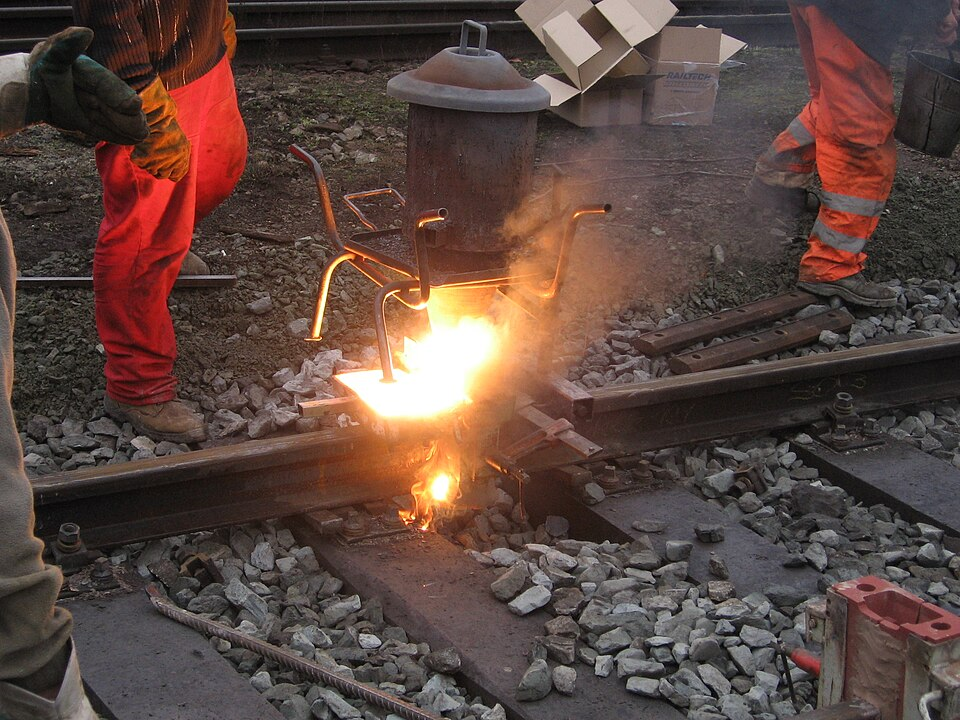
\includegraphics[width=0.5\linewidth]{images/book3/thermite.jpg}

{\small Soldagem aluminotérmica de um trilho: a reação do óxido de ferro com
o alumínio no cadinho acima da junta dá ferro líquido, que escorre para o
molde entre as duas pontas do trilho. (Fotografia: PetrS., CC BY-SA 3.0,
Wikimedia Commons.)}
\end{omfigure}

\section{O carbono e o monóxido de carbono}

Três retas envolvem o carbono:
\begin{itemize}
  \item \ce{C + O2 -> CO2}: um mol de gás dá um, $\Delta_r S^\circ
        \approx 0$, uma reta quase horizontal perto de \qty{-395}{kJ};
  \item \ce{2C + O2 -> 2CO}: um mol de gás dá dois, $\Delta_r S^\circ
        \approx \qty{+180}{J/(K.mol)}$, uma reta que \emph{desce} com a temperatura;
  \item \ce{2CO + O2 -> 2CO2}: três mols de gás dão dois, uma reta ascendente.
\end{itemize}

\begin{proposition}[A quente, o carbono reduz quase tudo]\label{prop:b2:ellingham:carbon}
A reta de \ce{2C + O2 -> 2CO} desce com a temperatura e cruza as retas da
maioria dos óxidos metálicos: acima da temperatura de cruzamento, o carbono
reduz o óxido, formando monóxido de carbono. O cruzamento com o óxido de
ferro(II) fica perto de \qty{1040}{K}, com o óxido de zinco perto de
\qty{1220}{K}; para o dióxido de titânio e a magnésia, fica perto de
\qty{2000}{K} ou acima, para a alumina ainda mais alto, onde os metais se
combinam com o carbono formando carbonetos ou se reoxidam quando o gás esfria.
\end{proposition}

\begin{proof}
A inclinação $-\Delta_r S^\circ$ da reta do carbono é negativa ($\Delta\nu_{\text{gás}}
= +1$), a das retas dos óxidos é positiva: elas se encontram uma vez. As
temperaturas são lidas nas retas calculadas.
% ledger: janafG:CO.900, janafG:CO.1100, janafG:FeO.900, janafG:FeO.1100 (crossings computed in figdata/bachelor-2/ellingham.py)
\end{proof}

\begin{definition}[Equilíbrio de Boudouard]\label{def:b2:ellingham:boudouard}
O \emph{equilíbrio de Boudouard}\index{equilibrio de Boudouard@equilíbrio de Boudouard} é \ce{C(s) + CO2(g) <=> 2CO(g)},
\omterm{def:b2:reaction-enthalpy:exothermic}{endotérmico}, entre o carbono e os dois óxidos de carbono.
\end{definition}

\begin{proposition}[Composição do gás sobre o carbono]\label{prop:b2:ellingham:boudouard}
O sistema carbono + \ce{CO} + \ce{CO2} tem \omterm{def:b2:equilibrium-shifts:variance}{variância} 2: a $T$ e pressão total
$p$ dadas, a fração molar $x$ do monóxido de carbono é fixada por $x^2/(1 - x)
= K^\circ(T)\,p^\circ/p$. A \qty{1}{bar}, o gás é quase \ce{CO2} puro
abaixo de \qty{700}{K} e quase \ce{CO} puro acima de \qty{1200}{K}; o
cruzamento das três retas do carbono, perto de \qty{975}{K}, é onde $K^\circ = 1$.
\end{proposition}

\begin{proof}
Três espécies, uma reação, duas fases: $v = 3 - 1 + 2 - 2 = 2$. Com $p_{\ce{CO}}
= xp$ e $p_{\ce{CO2}} = (1 - x)p$, $Q = x^2p/[(1 - x)p^\circ]$. Em $K^\circ = 1$,
as \omterm{def:b2:reaction-free-energy:gibbs-energy}{energias de Gibbs} padrão de \ce{2C + O2 -> 2CO} e de \ce{C + O2 -> CO2} são
iguais: as duas retas, e portanto a terceira, se encontram.
\end{proof}

\begin{omfigure}
\begin{tikzpicture}
\begin{axis}[
  width=0.62\linewidth, height=5.4cm, xmin=500, xmax=1500, ymin=0, ymax=1.05,
  axis x line=bottom, axis y line=left, xlabel={$T$ (K)},
  xtick={500,700,900,1100,1300,1500}, ytick={0,0.5,1},
  ylabel={fração molar de \ce{CO}}, tick label style={font=\small},
  label style={font=\small}, clip=false]
\addplot[omThm, very thick] table[x=T, y=xCO] {figdata/out/bachelor-2-ellingham-b.dat};
\node[font=\scriptsize, anchor=west] at (axis cs:1150,0.55) {\ce{CO} estável};
\node[font=\scriptsize, anchor=west] at (axis cs:510,0.6) {\ce{CO2} (e carbono) estável};
\end{axis}
\end{tikzpicture}

{\small O \omterm{def:b2:ellingham:boudouard}{equilíbrio de Boudouard} a \qty{1}{bar}: fração molar de monóxido de
carbono em um gás em equilíbrio com o carbono.}
% ledger: janafG:CO.700, janafG:CO2.700, janafG:CO.1100, janafG:CO2.1100 (computed in figdata/bachelor-2/ellingham.py)
\end{omfigure}

\section{O alto-forno}

O minério de ferro (hematita \ce{Fe2O3}, magnetita \ce{Fe3O4}), o coque e o
calcário são carregados no topo de uma cuba alta; ar quente é soprado
perto da base. Ao descer, os sólidos encontram um gás quente ascendente; o gás
sai pelo topo, resfriado.
\begin{itemize}
  \item Nas ventaneiras, o coque queima no ar quente: \ce{C + O2 -> CO2} e,
        acima, com excesso de carbono, \ce{CO2 + C -> 2CO} (Boudouard): o gás
        que sobe é sobretudo monóxido de carbono e nitrogênio.
  \item Na parte superior, o monóxido de carbono reduz os óxidos de ferro
        etapa por etapa, \ce{3Fe2O3 + CO -> 2Fe3O4 + CO2}, \ce{Fe3O4 + CO -> 3FeO + CO2},
        \ce{FeO + CO -> Fe + CO2}. As duas primeiras etapas são fáceis; para a
        última, a reta \ce{CO}/\ce{CO2} passa um pouco \textit{acima} da reta
        do \ce{FeO}: sua \omterm{def:b2:reaction-free-energy:reaction-gibbs}{energia de Gibbs padrão de reação} é ligeiramente
        positiva ($K^\circ \approx 0.3$ a \qty{900}{K}), e a redução exige um
        gás com pelo menos três vezes mais \ce{CO} que \ce{CO2} --- o que o
        \omterm{def:b2:ellingham:boudouard}{equilíbrio de Boudouard} fornece na zona quente logo abaixo.
  \item Mais abaixo e mais quente, o próprio carbono reduz o que resta, \ce{FeO + C ->
        Fe + CO}; o ferro dissolve carbono, funde e se acumula no fundo
        com uma escória fundida formada pela cal e pela sílica do minério.
\end{itemize}

\begin{omfigure}
\begin{tikzpicture}[font=\small, >={Stealth}]
  \fill[gray!12] (-1.4,0) -- (-2.0,3.0) -- (-1.3,7.0) -- (1.3,7.0) -- (2.0,3.0) -- (1.4,0) -- cycle;
  \draw[thick] (-1.4,0) -- (-2.0,3.0) -- (-1.3,7.0) (1.4,0) -- (2.0,3.0) -- (1.3,7.0);
  \draw[thick] (-1.4,0) -- (1.4,0);
  \fill[orange!70!red] (-1.4,0) rectangle (1.4,0.35);
  \fill[yellow!50!orange] (-1.45,0.35) rectangle (1.45,0.6);
  \node[font=\scriptsize] at (0,0.17) {ferro líquido};
  \node[font=\scriptsize] at (0,0.48) {escória};
  % tuyeres
  \draw[->, thick, omDef] (-3.2,1.2) -- (-1.75,1.2) node[pos=0, left] {ar quente};
  \draw[->, thick, omDef] (3.2,1.2) -- (1.75,1.2);
  % charge and gas
  \draw[->, thick] (-0.6,7.9) -- (-0.6,7.1) node[pos=0, above left, xshift=6pt] {minério, coque, calcário};
  \draw[->, thick, omThm] (0.7,7.1) -- (0.7,7.9) node[pos=1, above right, xshift=-6pt] {gás de topo (\ce{CO}, \ce{CO2}, \ce{N2})};
  \draw[->, omThm, thick] (0.6,1.6) -- (0.6,6.4);
  \draw[->, thick] (-0.6,6.4) -- (-0.6,1.6);
  \node[omThm, font=\scriptsize, rotate=90] at (0.9,4.0) {o gás sobe};
  \node[font=\scriptsize, rotate=90] at (-0.9,4.0) {os sólidos descem};
  % zones
  \node[anchor=west, align=left, font=\scriptsize] at (2.3,6.0) {\ce{3Fe2O3 + CO -> 2Fe3O4 + CO2}\\ \ce{Fe3O4 + CO -> 3FeO + CO2}};
  \node[anchor=west, align=left, font=\scriptsize] at (2.3,4.2) {\ce{FeO + CO -> Fe + CO2}};
  \node[anchor=west, align=left, font=\scriptsize] at (2.3,2.7) {\ce{CO2 + C -> 2CO}\\ \ce{FeO + C -> Fe + CO}};
  \node[anchor=west, align=left, font=\scriptsize] at (2.3,1.6) {\ce{C + O2 -> CO2}};
  \draw[densely dotted] (1.95,6.0) -- (2.3,6.0) (1.9,4.2) -- (2.3,4.2) (2.0,2.8) -- (2.3,2.8);
  \node[anchor=east, align=right, font=\scriptsize, black!60] at (-2.2,6.0) {mais frio};
  \node[anchor=east, align=right, font=\scriptsize, black!60] at (-2.2,2.3) {mais quente};
  \draw[->, black!50] (-2.6,5.6) -- (-2.6,2.7);
\end{tikzpicture}

{\small O alto-forno como reator em contracorrente. Os sólidos descem, o gás
redutor quente sobe; os óxidos de ferro são reduzidos pelo monóxido de
carbono na parte superior, mais fria, e pelo carbono na parte inferior, mais
quente. O ferro e a escória são extraídos pelo fundo.}
\end{omfigure}

\begin{omfigure}
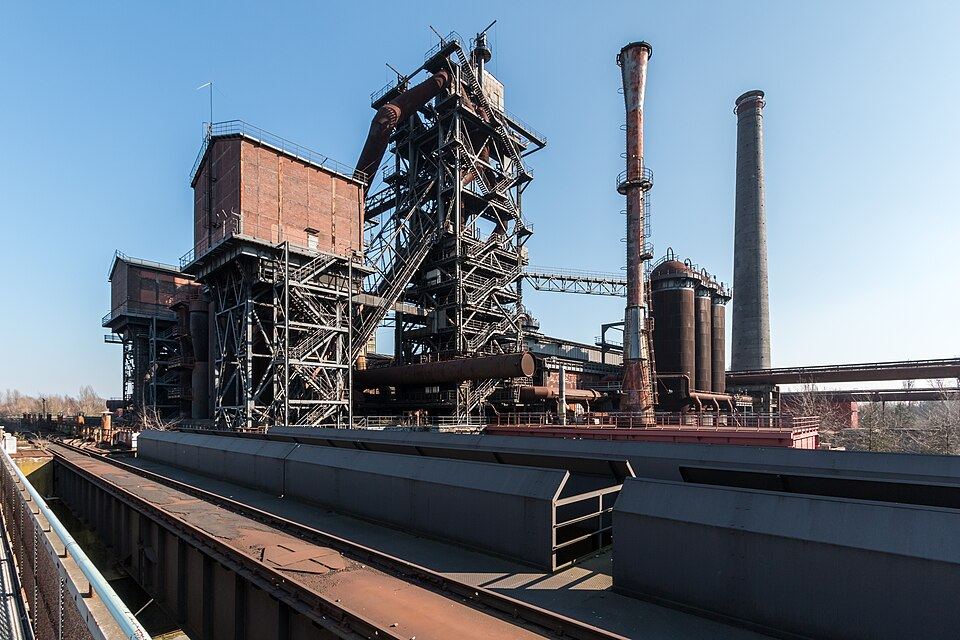
\includegraphics[width=0.6\linewidth]{images/book3/blast-furnace.jpg}

{\small Um alto-forno preservado como monumento (Duisburg-Nord, desativado em
1985): a cuba alta com seu anel de tubulações para o ar quente e as tomadas
de gás no topo. (Fotografia: Dietmar Rabich, CC BY-SA 4.0, Wikimedia Commons.)}
\end{omfigure}

\section{Outras vias para obter um metal}

\begin{definition}[Pirometalurgia e hidrometalurgia]\label{def:b2:ellingham:metallurgy}
A \emph{pirometalurgia}\index{pirometalurgia} extrai um metal a alta
temperatura, por redução de seu óxido em um forno. A \emph{hidrometalurgia}\index{hidrometalurgia}
o extrai de uma solução aquosa. Suas etapas usuais são a
\emph{ustulação}\index{ustulacao@ustulação} (aquecer um minério sulfetado ao ar para
transformá-lo em óxido, \ce{2ZnS + 3O2 -> 2ZnO + 2SO2}), a \emph{lixiviação}\index{lixiviacao@lixiviação}
(dissolver o composto do metal, muitas vezes em ácido sulfúrico, \ce{ZnO + 2H+ ->
Zn^2+ + H2O}), a purificação da solução, por exemplo por
\emph{cementação}\index{cementacao@cementação} (redução dos íons de um metal mais nobre
por um pó de um metal menos nobre, \ce{Cu^2+ + Zn -> Cu + Zn^2+}), e a
recuperação do metal, muitas vezes por eletrólise.
\end{definition}

O diagrama explica a divisão do trabalho. Ferro, zinco, chumbo e estanho são
obtidos com carbono em um forno. O alumínio, cuja reta fica muito abaixo da
do carbono em qualquer temperatura praticável, é produzido por eletrólise de
seu óxido fundido (\cref{ch:b2:batteries-electrolysis}); o magnésio, por
eletrólise ou por redução com silício sob vácuo, que retira o vapor de
magnésio; o titânio, convertendo o óxido em cloreto, \ce{TiO2 + 2Cl2 + C -> TiCl4 +
CO2} (\cref{exo:b2:reaction-free-energy:12}), e depois reduzindo o cloreto com
magnésio (o processo Kroll). A maior parte do zinco do mundo é produzida por
\omterm{def:b2:ellingham:metallurgy}{ustulação}, \omterm{def:b2:ellingham:metallurgy}{lixiviação} e eletrólise: a via hidrometalúrgica dá um metal mais
puro e evita manipular vapor de zinco.

\begin{omfigure}
\begin{tikzpicture}[font=\small, >={Stealth}, box/.style={draw, thick, rounded corners=2pt, align=center, minimum height=0.9cm, fill=white, text width=2.3cm}]
  \node[box] (r) at (0,0) {ustulação\\ \ce{ZnS} $\to$ \ce{ZnO}};
  \node[box] (l) at (3.2,0) {lixiviação\\ em \ce{H2SO4}};
  \node[box] (c) at (6.4,0) {purificação\\ (cementação)};
  \node[box] (e) at (9.6,0) {eletrólise\\ \ce{Zn^2+} $\to$ \ce{Zn}};
  \draw[->, thick] (r) -- (l); \draw[->, thick] (l) -- (c); \draw[->, thick] (c) -- (e);
  \draw[->, thick, black!60] (r.north) -- ++(0,0.7) node[above] {\ce{SO2} $\to$ ácido sulfúrico};
  \draw[->, thick, omThm] (e.south) -- ++(0,-0.6) -| (l.south) node[pos=0.25, below] {ácido devolvido};
  \draw[->, thick] (e.east) -- ++(0.8,0) node[right] {zinco};
\end{tikzpicture}

{\small A via hidrometalúrgica do zinco. O dióxido de enxofre do ustulador
é transformado no ácido sulfúrico da \omterm{def:b2:ellingham:metallurgy}{lixiviação}; o ácido regenerado no
ânodo da eletrólise é devolvido a ela.}
\end{omfigure}

\section{Exercícios}

\begin{exercise}[$\star$]\label{exo:b2:ellingham:1}
Escreva as reações representadas pelas retas do óxido de cobre(I), da alumina,
do monóxido de carbono e do dióxido de carbono, cada uma para um mol de \ce{O2}.
\end{exercise}

\begin{exercise}[$\star$]\label{exo:b2:ellingham:2}
A partir dos valores-chave do CODATA ($\Delta_f H^\circ(\ce{ZnO}) = \qty{-350.46}{kJ/mol}$,
$S^\circ$: \ce{ZnO} 43.65, \ce{Zn} 41.63, \ce{O2} \qty{205.15}{J/(K.mol)}),
escreva $\Delta_r G^\circ(T)$ de \ce{2Zn + O2 -> 2ZnO} para o zinco sólido.
\end{exercise}

\begin{exercise}[$\star$]\label{exo:b2:ellingham:3}
Usando o diagrama, liste os metais que podem reduzir o óxido de cromo(III) a
\qty{1500}{K} e os que não podem.
\end{exercise}

\begin{exercise}[$\star$]\label{exo:b2:ellingham:4}
Explique o sinal da inclinação de cada uma das três retas do carbono.
\end{exercise}

\begin{exercise}[$\star\star$]\label{exo:b2:ellingham:5}
Calcule a \omterm{def:b2:ellingham:oxygen-pressure}{pressão de oxigênio de equilíbrio} do óxido de mercúrio(II) a \qty{600}{K}
(mercúrio líquido, $\Delta_r H^\circ = \qty{-181.6}{kJ}$, $\Delta_r S^\circ =
\qty{-216.5}{J/K}$ por mol de \ce{O2}). O mercúrio é oxidado no ar a essa
temperatura?
\end{exercise}

\begin{exercise}[$\star\star$]\label{exo:b2:ellingham:6}
Calcule $\Delta_r G^\circ$ a \qty{298}{K} da reação da termita, \ce{Fe2O3 +
2Al -> Al2O3 + 2Fe}, dados $\Delta_f G^\circ = \qty{-743.5}{kJ/mol}$ para
\ce{Fe2O3} e \qty{-1582.3}{kJ/mol} para \ce{Al2O3}, e diga por que a reação,
embora muito \omterm{def:b2:reaction-free-energy:exergonic}{exergônica}, não começa à temperatura ambiente.
% ledger: janafG:Fe2O3.298, janafG:Al2O3.298
\end{exercise}

\begin{exercise}[$\star\star$]\label{exo:b2:ellingham:7}
Encontre no diagrama a temperatura acima da qual o carbono reduz o óxido de
ferro(II) a ferro com formação de monóxido de carbono, e escreva a reação.
\end{exercise}

\begin{exercise}[$\star\star$]\label{exo:b2:ellingham:8}
A \qty{1100}{K}, $\Delta_f G^\circ(\ce{CO}) = \qty{-209.1}{kJ/mol}$ e
$\Delta_f G^\circ(\ce{CO2}) = \qty{-396.0}{kJ/mol}$. Calcule o $K^\circ$ do
\omterm{def:b2:ellingham:boudouard}{equilíbrio de Boudouard} e a fração molar de monóxido de carbono sobre o
carbono a \qty{1}{bar}. O que acontece com o gás, em contato com fuligem ou
com ferro, quando ele é resfriado a \qty{700}{K}?
% ledger: janafG:CO.1100, janafG:CO2.1100
\end{exercise}

\begin{exercise}[$\star\star$]\label{exo:b2:ellingham:9}
O hidrogênio é às vezes usado para reduzir o óxido de tungstênio. Usando a reta
da água, explique por que o hidrogênio é um redutor melhor que o monóxido de
carbono a alta temperatura, mas pior a baixa temperatura.
\end{exercise}

\begin{exercise}[$\star\star\star$]\label{exo:b2:ellingham:10}
O óxido de magnésio pode ser reduzido pelo silício, \ce{2MgO + Si -> SiO2 + 2Mg}, embora
a reta da sílica fique acima da reta da magnésia em todas as temperaturas do
diagrama. A \qty{1500}{K}, o magnésio é um gás e as tabelas dão, por mol de
\ce{O2}, \qty{-845.5}{kJ} para a magnésia e \qty{-643.7}{kJ} para a sílica.
Calcule o $\Delta_r G^\circ$ da redução e depois a pressão de vapor de
magnésio abaixo da qual ela ocorre no sentido direto. Como um forno a vácuo
aproveita isso?
% ledger: janafG:MgO.1500, janafG:SiO2.1500
\end{exercise}

\begin{exercise}[$\star\star\star$]\label{exo:b2:ellingham:11}
Calcule a \omterm{def:b2:equilibrium-shifts:variance}{variância} do sistema \ce{FeO(s)}, \ce{Fe(s)}, \ce{CO(g)},
\ce{CO2(g)} em equilíbrio. O que isso significa para o gás que sai da parte
superior de um alto-forno?
\end{exercise}

\begin{exercise}[$\star\star\star$]\label{exo:b2:ellingham:12}
O cobre é purificado de sua solução de \omterm{def:b2:ellingham:metallurgy}{lixiviação} por \omterm{def:b2:ellingham:metallurgy}{cementação} com sucata
de ferro. Usando os potenciais padrão do volume do 1.º ano ($E^\circ(\ce{Cu^2+}/\ce{Cu})
= \qty{0.34}{V}$, $E^\circ(\ce{Fe^2+}/\ce{Fe}) = \qty{-0.41}{V}$), calcule a
constante de equilíbrio de \ce{Cu^2+ + Fe -> Cu + Fe^2+} e a concentração
residual de íons cobre quando a solução contém \qty{1.0}{mol/L} de
\ce{Fe^2+}.
\end{exercise}

\section{Problema: O zinco pelo fogo}

\begin{problem}[{Problema de fim de semana --- as retas de Ellingham do óxido de
zinco e do monóxido de carbono, a temperatura na qual o carbono reduz o óxido
de zinco, a variância do forno e a condensação do vapor de zinco}]
\label{pb:b2:ellingham:1}
Antes da eletrólise, o zinco era produzido aquecendo seu óxido com carbono em
retortas de argila. Dados (CODATA e a tabela JANAF do zinco): $\Delta_f H^\circ(\ce{ZnO})
= \qty{-350.46}{kJ/mol}$; $S^\circ$ (\unit{J/(K.mol)}): \ce{ZnO} 43.65, \ce{Zn}
41.63, \ce{O2} 205.15; o zinco funde a \qty{692.7}{K} ($\Delta_{\text{fus}}H =
\qty{7.32}{kJ/mol}$) e ferve a \qty{1180.2}{K} sob \qty{1}{bar}
($\Delta_{\text{vap}}H = \qty{115.3}{kJ/mol}$). Para \ce{2C + O2 -> 2CO}, as
tabelas dão $\Delta_r G^\circ = \qty{-418.2}{kJ}$ a \qty{1100}{K} e
\qty{-453.0}{kJ} a \qty{1300}{K}.
% ledger: dfh:ZnO_cr, s0:ZnO_cr, s0:Zn_cr, s0:O2_g, hT:Zn_cr.692, hT:Zn_l.692, hT:Zn_l.1180, hT:Zn_g.1180, dfh:Zn_g, janafG:CO.1100, janafG:CO.1300

\medskip
\noindent\textbf{Parte I --- A reta do óxido de zinco.}
\begin{enumerate}
  \item Calcule $\Delta_r H^\circ$ e $\Delta_r S^\circ$ de \ce{2Zn(s) + O2 ->
        2ZnO} a \qty{298}{K}.
  \item Escreva $\Delta_r G^\circ(T)$ abaixo do ponto de fusão.
  \item Calcule as entropias de fusão e de vaporização do zinco.
  \item Escreva $\Delta_r G^\circ(T)$ entre os pontos de fusão e de ebulição.
  \item Escreva-a acima do ponto de ebulição.
  \item Calcule as três inclinações e explique por que a última é muito mais acentuada.
  \item Verifique que as três expressões concordam nas temperaturas de transição.
\end{enumerate}

\medskip
\noindent\textbf{Parte II --- A reta do carbono.}
\begin{enumerate}[resume]
  \item A partir dos dois valores tabelados, escreva a reta de \ce{2C + O2 -> 2CO} na
        forma $a + bT$ entre \qty{1100}{K} e \qty{1300}{K}.
  \item Deduza seu $\Delta_r S^\circ$ e explique seu sinal.
  \item Escreva a redução \ce{ZnO + C -> Zn(g) + CO} e seu $\Delta_r
        G^\circ(T)$ como diferença das duas retas (por mol de \ce{O2}).
  \item Encontre a temperatura em que as duas retas se cruzam.
  \item Por que é importante que essa temperatura esteja acima do ponto de
        ebulição do zinco?
\end{enumerate}

\medskip
\noindent\textbf{Parte III --- A retorta.}
\begin{enumerate}[resume]
  \item Calcule a \omterm{def:b2:equilibrium-shifts:variance}{variância} do sistema \ce{ZnO(s)}, \ce{C(s)}, \ce{Zn(g)},
        \ce{CO(g)}, com o zinco e o monóxido de carbono formados apenas pela redução.
  \item Em uma retorta a \qty{1300}{K} sob \qty{1}{bar}, quais são as pressões
        parciais do zinco e do monóxido de carbono se a reação for completa?
  \item Calcule o $\Delta_r G^\circ$ da redução a \qty{1300}{K} e o
        $K^\circ$ correspondente.
  \item Explique por que a retorta é operada um pouco acima da temperatura de
        cruzamento, e não muito acima dela.
\end{enumerate}

\medskip
\noindent\textbf{Parte IV --- O condensador.}
\begin{enumerate}[resume]
  \item O vapor é conduzido a um condensador mais frio. Escreva a reação pela
        qual o vapor de zinco pode ser reoxidado pelo dióxido de carbono.
  \item Usando o diagrama, explique por que o gás deve ser mantido isento de
        dióxido de carbono.
  \item Por que o zinco deve ser condensado depressa, e não lentamente?
  \item Calcule a massa de carbono necessária por tonelada de zinco,
        tomando a redução tal como está escrita.
  \item Calcule o calor absorvido por tonelada de zinco pela redução a cerca
        de \qty{1300}{K} (tome $\Delta_r H^\circ$ das expressões das Partes I
        e II).
  \item Dê a temperatura acima da qual o carbono reduz o óxido de zinco em
        condições padrão.
\end{enumerate}
\end{problem}
